%
% dual.tex -- duale frames
%
% (c) 2019 Prof Dr Andreas Müller, Hochschule Rapperswil
%
\section{Das duale Frame\label{section:dual}}
\rhead{Das duale Frame}
In diesem Abschnitt gehen wird davon aus, dass $\mathcal{B}$ ein
Frame in $\mathbb{R}^n$ ist mit Framekonstanten $A$ und $B$.

\subsection{Frame-Operator\label{subsection:frame-operator}}
Der Frame-Operator berechnet die Analysekoeffizienten
$\hat{v}_k=\langle v,b_k\rangle$ eines Signals
$v\in \mathbb R^n$ bezüglich des Frames $\mathcal{B}$:
\[
\mathcal{T}\colon \mathbb R^n \to \mathbb R^m
:
v \mapsto
\begin{pmatrix}
\hat{v}_1\\\hat{v}_2\\\vdots\\\hat{v}_m
\end{pmatrix}
=
(\hat{v}_k=\langle v,b_k\rangle)_{1\le k\le m}.
\]
Zur Berechnung der Skalarprodukte kann man das Matrizenproukt
\[
\langle v,b_k\rangle
=
b_k^t v
\]
verwenden.
Die Zeilenvektoren $b_k^t$ kann man zeilenweise in einer grossen Matrix $T$
\[
T 
=
\begin{pmatrix}
\dots&b_1^t &\dots\\
\dots&b_2^t &\dots\\
     &\vdots&     \\
\dots&b_m^t &\dots
\end{pmatrix}
\]
zusammenführen.
Das Matrixprodukt $Tv$ liefert dann genau das Resultat des Frame-Operators
\[
\mathcal{T} v
=
\begin{pmatrix}
\langle v, b_1\rangle\\
\langle v, b_2\rangle\\
\vdots\\
\langle v, b_m\rangle\\
\end{pmatrix}
=
\begin{pmatrix}
b_1^tv\\
b_2^tv\\
\vdots\\
b_m^tv\\
\end{pmatrix}
=
\begin{pmatrix}
\dots&b_1^t &\dots\\
\dots&b_2^t &\dots\\
     &\vdots&     \\
\dots&b_m^t &\dots
\end{pmatrix}
v
=
Tv.
\]
Die Matrix $T$ ist die Matrix des Frame-Operator $\mathcal T$ bezüglich der
Standardbasis von $\mathbb R^n$.

\begin{beispiel}
Im Beispiel von Abschnitt~\ref{subsection:hexagon} besteht das Frame
aus den Vektoren
\[
\mathcal{B}
=
\biggl\{
\begin{pmatrix}1\\[2pt] 0\end{pmatrix},
\begin{pmatrix}-\frac12\\[2pt] \frac{\sqrt{3}}2\end{pmatrix},
\begin{pmatrix}-\frac12\\[2pt] -\frac{\sqrt{3}}2\end{pmatrix}
\biggr\}.
\]
Der zugehörige Frameoperator $\mathcal{T}$ hat daher die Matrix
\begin{equation}
T
=
\begin{pmatrix}
1&0\\[2pt]
-\frac12&\frac{\sqrt{3}}2\\[2pt]
-\frac12&-\frac{\sqrt{3}}2
\end{pmatrix}.
\label{beispielTmatrix}
\end{equation}
\end{beispiel}

\subsubsection{Die Gram-Matrix}
Das Frame $\mathcal{B}$ mit den Frame-Konstanten $A$ und $B$ erfüllt
\[
A\|v\|^2 \le \sum_{k=1}^m |\langle v,b_k\rangle|^2 \le B\|v\|^2
\qquad\forall v\in \mathbb R^n.
\]
Die Quadratsumme in der Mitte ist genau die Norm des Vektors
$\mathcal{V}$ in $\mathbb R^m$.
Unterscheiden wir für den Moment die verschiedenen Skalarprodukte
und Normen dadurch, dass wir die Vektorräume als Indizes hinzufügen,
können wir die Frame-Ungleichung schreiben als
\[
A \| v\|_{\mathbb R^n}^2
\le
\| Tv\|_{\mathbb R^m}^2
\le
B \| v\|_{\mathbb R^n}^2.
\]
Die Norm von $Tv$ in $\mathbb R^m$ ist
\[
\| Tv\|_{\mathbb R^m}^2
=
\langle Tv,Tv\rangle_{\mathbb R^m}
=
(Tv)^tTv
=
v^t(T^tT)v
=
\langle T^tTv,v\rangle_{\mathbb R^n}.
\]
Man beachte, dass $T^tT$ eine symmetrische $n\times n$-Matrix ist,
die codiert, wie stark die einzelnen Vektoren $v\in\mathbb R^n$ durch
den Frame-Operator $\mathcal{T}$ verzerrt werden.
Dies rechtfertigt eine eigene Definition.

\begin{definition}
Ist $T$ die Matrix des Frame-Operators $\mathcal{T}$ eines Frames
$\mathcal{B}$, dann heisst $G=T^tT$ der Gram-Operator des Frames
$\mathcal{B}$.
\end{definition}

Die Frame-Bedingung lässt sich mit dem Gram-Operator $T^tT$ als
\begin{equation}
A \|v\|^2
\le
\langle T^t T v,v\rangle
\le
B \|v\|^2
\label{framebedingung:ttt}
\end{equation}
schreiben.
Man kann daraus schliessen, dass der Gram-Operator $T^tT$ regulär ist.

Die symmetrische Matrix $T^tT$ kann durch Wahl einer geeigneten Basis
in $\mathbb R^n$ diagonalisiert werden.
Die Eigenvektoren können sogar orthonormiert gewählt werden.
Seien daher $u_1,\dots,u_n$ Eigenvektoren von $T^tT$ mit Eigenwerten
$\lambda_1\le\dots\le\lambda_n$.
Die Framebedingung~\eqref{framebedingung:ttt}
für den Vektore $v=u_k$ sagt dann
\[
A \| u_k\|^2
=
A
\le
\langle T^tTu_k,u_k\rangle
=
\lambda_k\langle u_k,u_k\rangle
=
\lambda_k
=
B \| u_k\|^2
=
B.
\]
Die Eigenwerte von $T^tT$ sind also alle zwischen $A$ und $B$.
Man kann sogar noch mehr sagen:

\begin{satz}
Sei $\mathcal{B}\subset\mathbb R^n$ eine Menge von Vektoren derart,
dass die zugehörige Matrix $T^tT$ regulär ist.
Seien weiter $\lambda_1\le\dots\le \lambda_n$ die Eigenwerte
(mit Vielfachheiten) von $T^tT$.
Dann ist $\mathcal{B}$ ein Frame mit Framekonstanten
$A=\lambda_1$ und $B=\lambda_n$.
\end{satz}

\begin{beispiel}
Im Beispiel von Abschnitt~\ref{subsection:hexagon} ist die Matrix $T$
gegeben in \eqref{beispielTmatrix}.
Der zugehörige Gram-Operator ist
\[
T^tT
=
\begin{pmatrix}
1& -\frac12        &-\frac12          \\[2pt]
0& \frac{\sqrt{3}}2& -\frac{\sqrt{3}}2
\end{pmatrix}
\begin{pmatrix}
1&0\\
-\frac12&\frac{\sqrt{3}}2\\[2pt]
-\frac12&-\frac{\sqrt{3}}2
\end{pmatrix}
=
\begin{pmatrix}
1+\frac14+\frac14 & 0-\frac{\sqrt{3}}4+\frac{\sqrt{3}}4\\[2pt]
0-\frac{\sqrt{3}}4+\frac{\sqrt{3}}4&0+\frac{3}{4}+\frac{3}{4}
\end{pmatrix}
=
\begin{pmatrix}
\frac32&0\\
0&\frac32
\end{pmatrix}
=
\frac{3}{2}E
\]
Da die Matrix $T^tT$ bereits diagonal ist, können die Eigenwerte
$\lambda_1=\lambda_2=\frac32$ direkt abgelesen werden.
\end{beispiel}

Das Frame des Beispiels ist straff und der Gram-Operator ist ein
Vielfaches der Einheitsmatrix.
Dies ist kein Zufall, wie das folgende Korollar zeigt.

\begin{korollar}
Das Frame $\mathcal{B}$ ist genau dann straff, wenn der zugehörige
Gram-Operator $T^tT$ ein Vielfaches der Einheitsmatrix ist.
\end{korollar}

\begin{figure}
\centering
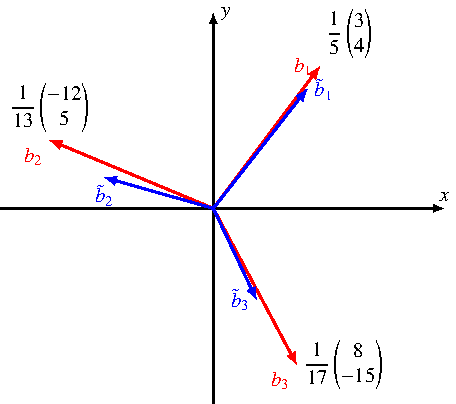
\includegraphics{chapters/1-geometrie/images/beispiel2.pdf}
\caption{Beispiel eines nicht straffen Frames mit rationalen Framevektoren
$b_k$ (rot).
Die Vektoren $\tilde{b}_k$ des dualen Frames
(siehe Definition~\ref{definition:dualesframe}) sind blau eingezeichnet.
\label{frame:beispiel2}}
\end{figure}

\begin{beispiel}
Die Vektoren
\[
\mathcal{B} 
=
\biggl\{
\frac15
\begin{pmatrix} 3\\4\end{pmatrix},
\frac1{13}
\begin{pmatrix} -12\\5\end{pmatrix},
\frac1{17}
\begin{pmatrix} 8\\-15\end{pmatrix}
\biggr\}
\subset \mathbb R^2
\]
erzeugen den ganzen Raum $\mathbb R^2$, sie bilden daher ein
Frame (Abbildung~\ref{frame:beispiel2}).
Wir berechnen den Frame-Operator, den Gram-Operator und seine Eigenwerte
um die Frame-Konstanten zu ermiteln.

Der Frame-Operator ist die Matrix
\[
T
=
\begin{pmatrix}
 \frac{ 3}{ 5}& \frac{ 4}{ 5}\\[2pt]
-\frac{12}{13}& \frac{ 5}{13}\\[2pt]
 \frac{ 8}{17}&-\frac{15}{17}
\end{pmatrix}.
\]
Der Gram-Operator wird daher
\[
G=T^tT
=
\begin{pmatrix}
 \frac{ 3}{ 5}&-\frac{12}{13}&  \frac{ 8}{17}\\[2pt]
 \frac{ 4}{ 5}& \frac{ 5}{13}& -\frac{15}{17}
\end{pmatrix}
\begin{pmatrix}
 \frac{ 3}{ 5}& \frac{ 4}{ 5}\\[2pt]
-\frac{12}{13}& \frac{ 5}{13}\\[2pt]
 \frac{ 8}{17}&-\frac{15}{17}
\end{pmatrix}
=
\frac{1}{1221025}
\begin{pmatrix}
1750369&  286808 \\
 286808& 1676106
\end{pmatrix}
\]
Die Eigenwerte dieser $2\times 2$-Matrix können als Nullstellen des
charakteristischen Polynoms mit der Lösungsformel für quadratische
Gleichungen berechnet werden.
Man findet zum Beispiel mit Hilfe eines Computer-Algebra-Systems
\[
\lambda_{\pm}
=
\frac{52715\pm 41\sqrt{47105}}{37570}
\quad\Rightarrow\quad
\left\{
\begin{aligned}
A&=
1.166262672548251
\\
B&=
1.639965701154171.
\end{aligned}
\right.
\]
Da die beiden Konstanten nicht übereinstimmen, ist dieses Frame
nicht straff.
\end{beispiel}

\begin{proof}[Beweis]
Ein straffes Frame hat $A=B$, was gleichbedeutend damit ist, dass
die Eigenwerte des Frame-Operators $T^tT$ mit 
$A=B=\lambda_1=\dots=\lambda_n$ übereinstimmen.
Dies wiederum ist gleichbedeutend damit, dass alle Vektoren Eigenvektoren
zum gleichen Eigenwert sind und $T^tT=AE=BE$.
\end{proof}

\subsubsection{Die inverse Abbildung des Frame-Operators}
Für ein straffes Frame gilt $T^tT  = AE$.
Bis auf den Faktor $A$ ist daher $T^t$ bereits eine Linksinverse von $T$.
Genauer, mit
\[
S=\frac1{A} T^t
\qquad\text{folgt}\qquad
ST
=
\frac1{A} T^tT
=
\frac1{A} AE
=
E.
\]
Eine Linksinverse von $\mathcal{T}$ ist also für ein straffes Frame
leicht zu finden.

Für ein beliebiges Frame lässt sich ebenfalls eine Linksinverse angeben.
Mit $G=T^tT$ ist
\[
v
=
\underbrace{G^{-1}T^t}_{\displaystyle=S}Tv
=
STv,
\]
die Matrix $S=G^{-1}T^t$ ist also die gesuchte Linksinverse von $T$.

\subsubsection{Das duale Frame}
Um den Frame-Operator umzukehren, muss man $G^{-1}T^t$ berechnen
können.
Auf einen Vektor $\hat{v} = (\hat{v}_k)_{1\le k\le m} = Tv$ angewendet
bedeutet dies, dass man $G^{-1}$ auf
\[
T^t \hat{v} = \sum_{k=1}^m \hat{v}_k  b_k,
\]
anwenden muss, dabei wurde verwendet, dass $T^t$ als Spalten die
Vektoren $b_k$ enthält.
Anwendung von $G^{-1}$ liefert
\[
v
=
G^{-1} T^t \hat{v}
=
\sum_{k=1}^m \hat{v}_k G^{-1}b_k.
\]
Den Vektor $v$ erhält man also als Linearkombination der Vektoren
\[
\tilde{\mathcal{B}}
=
\{ G^{-1}b_1,\dots,G^{-1}b_n\}
=
\{ \tilde{b}_k = G^{-1}b_k\,|\, 1\le k\le m\}.
\]

\begin{definition}
\label{definition:dualesframe}
Ist $\mathcal{B}=\{b_1,\dots,b_m\}$, dann heisst
$\tilde{\mathcal{B}} = \{\tilde{b}_1,\dots,\tilde{b}_m\}$ 
mit
$\tilde{b}_k=G^{-1} b_k$
das zu $\mathcal{B}$ duale Frame.
\end{definition}

\begin{beispiel}
Das duale Frame zum Beispiel zu Abbildung~\ref{frame:beispiel2} kann
ebenfalls mit Hilfe eines Computer-Algebra-Systems berechnet werden aus
der bereits früher berechneten Matrix bestimmt werden.
Aus 
\[
G^{-1}T^t
=
\begin{pmatrix}
\frac{4259}{8053}
	&-\frac{718432}{1167685}
		&\frac{284716}{1167685}\\[2pt]
\frac{5422}{8053}
	&\frac{408473}{2335370}
		&-\frac{1203549}{2335370}
\end{pmatrix}
=
\begin{pmatrix}
0.52887&-0.61526&\phantom{-} 0.24383\\
0.67329&\phantom{-} 0.17490&-0.51536
\end{pmatrix}
\]
findet man das duale Frame
\[
\tilde{\mathcal{B}}
=
\left\{
\begin{pmatrix}
\frac{4259}{8053}\\[2pt]
\frac{5422}{8053}
\end{pmatrix},
\begin{pmatrix}
-\frac{718432}{1167685}\\[2pt]
\frac{408473}{2335370}
\end{pmatrix},
\begin{pmatrix}
\frac{284716}{1167685}\\[2pt]
-\frac{1203549}{2335370}
\end{pmatrix}
\right\}
=
\left\{
\begin{pmatrix} 0.52887\\ 0.67329 \end{pmatrix},
\begin{pmatrix}-0.61526\\ \phantom{-}0.17490 \end{pmatrix},
\begin{pmatrix}\phantom{-}0.24383\\ -0.51536 \end{pmatrix}
\right\}.
\]
Die Vektoren des dualen Frames sind in Abbildung~\ref{frame:beispiel2}
blau eingezeichnet.
\end{beispiel}

\begin{korollar}
Ist $\mathcal{B}=\{b_1,\dots,b_m\}$ ein straffes Frame mit Framekonstanten
$A=B$, dann ist
\[
\tilde{\mathcal{B}}
=
\biggl\{\tilde{b}_k = \frac1Ab_k\,\bigg|\,1\le k\le m\biggr\}
\]
das dazu duale Frame.
\end{korollar}

\begin{proof}[Beweis]
Für ein straffes Frame ist $T^tT=AE$, also ist $G^{-1}=\frac1A E$.
Die Vektoren des dualen Frames sind daher
$\tilde{b}_k = \frac1AEb_k=\frac1Ab_k$.
\end{proof}

Die Linksinverse $S$ von $\mathcal{T}$ kann mit Hilfe des dualen Frames
sehr leicht formuliert werden.

\begin{satz}
Ist $\mathcal{B}$ ein Frame und $\tilde{\mathcal{B}}$ das dazu duale
Frame und ist $\hat{v} = Tv$, dann ist die Linksinverse $S$ von $T$
gegeben durch
\[
v
=
S\hat{v}
=
\sum_{k=1}^m \hat{v}_k \tilde{b}_k.
\]
Linearkombination der Vektoren des dualen Frames mit den Analysekoeffizienten
$\hat{v}_k$ liefert also das ursprüngliche Signal zurück.
\end{satz}

\begin{beispiel}
\label{beispiel3}
In diesem Beispiel betrachten wir das Frame bestehend aus den
Signalen, die auf einem von maximal zehn Samles konstant sind
und sonst verschwinden.
Das Signal $b_k$ verschwindet für Samples $i>k$ und $i<k-10$
und ist so normiert, dass $\|b_k\|=1$.
Die zugehörigen dualen Signale können direkt berechnet werden,
zwei Beispiele sind in den Abbildungen \ref{b3-01} und \ref{b3-05}
dargestellt.
\def\beispieldrei#1#2{
\begin{figure}
\centering
\includegraphics{chapters/1-geometrie/images/b3-#1.pdf}
\caption{Signal $b_{#2}$ aus dem Beispiel von Seite~\pageref{beispiel3}
und zugehöriges duales Signal $\tilde{b}_{#2}$.
\label{b3-#1}}
\end{figure}
}
\beispieldrei{01}{1}
%\beispieldrei{02}{3}
%\beispieldrei{03}{6}
%\beispieldrei{04}{10}
\beispieldrei{05}{20}
%\beispieldrei{06}{30}
%\beispieldrei{07}{40}
%\beispieldrei{08}{50}
%\beispieldrei{09}{60}
%\beispieldrei{10}{70}
\end{beispiel}

In der Definition~\ref{definition:dualesframe} wird das duale Frame
definiert ohne zu rechtfertigen, dass die Vektoren $\tilde{b}_k$ 
tatsächlich ein Frame bilden.
Wegen $b_k=G\tilde{b}_k$ ist aber klar, dass die Vektoren $\tilde{b}_k$
den ganzen Vektorraum $\mathbb R^n$ erzeugen.
Insbesondere bilden sie ein Frame.
Damit sind die Framekonstanten noch nicht bestimmt.
Dies wird im folgenden Satz nachgeholt.

\begin{satz}
Ist $\mathcal{B}=\{b_1,\dots,b_m\}$ ein Frame mit Framekonstanten
$A$ und $B$, dann hat das duale Frame die Framekonstanten $1/B$ und $1/A$.
\end{satz}

\begin{proof}[Beweis]
Um die Frame-Konstanten des dualen Frames zu bestimmen,
müssen der Frame-Operator $\tilde{T}$ und Gram-Operator $\tilde{G}$
des dualen Frames bestimmt werden.
Das duale Frame besteht aus den Spaltenvektoren von $S=G^{-1}T^t$,
also ist der Frameoperator $\tilde{T}=S^t$ und damit ist der Gram-Operator
\[
\tilde{G}
=
\tilde{T}^t\tilde{T}
=
(S^t)^tS^t
=
SS^t
=
G^{-1}T^tTG^{-1}
=
G^{-1}.
\]
Der Gram-Operator des dualen Frames ist daher die Inverse des
Gram-Operators des ursprünglichen Frames.
Sind $A=\lambda_1\le \dots\le \lambda_n=B$ die Eigenwerte  von $G$,
dann sind
$1/B\le \lambda_n^{-1} \le \dots \le \lambda_1^{-1}\le 1/A$ 
die Eigenwerte von $\tilde{G}=G^{-1}$.
Daraus folgen die behaupteten Framekonstanten.
\end{proof}

%
% Allgemeine Frames
%
\subsection{Allgemeine Frames}
Die Wahl der Indexmenge $K$ in der Definition~\ref{definition:frame}
war einigermassen willkürlich.
Schon bei der Fouriertransformation ist eine solche diskrete Menge
für die Indizierung der Vergleichsfunktionen nicht mehr ausreichend.
Dort werden nämlich die Funktion $e^{i\omega t}$ mit $\omega\in\mathbb R$
verwendet.
Auch die geplante Anwendung auf Wavelets ist davon betroffen.
Dort wollen wir mit Funktionen $\psi_{a,b}$ vergleichen, die 
skalierte und verschobene Versionen eines Mutter-Wavelets $\psi$ sind,
mit Skalierungsfaktor $a\in\mathbb R^*$ und $b\in \mathbb R$.

Lässt man eine beliebige Indexmenge zu, ist die Definition der
Transformation $T$
\[
k
\mapsto
(Tv)(k) = \langle v,e_k\rangle
\]
als komplexwertige Funktion auf $K$ immer noch sinnvoll.
Für eine überabzählbare Indexmenge $K$ ist die Summe 
\[
\sum_{k\in K} |\langle v,e_k\rangle|^2,
\]
die in der Definition eines Frames auftritt, schlicht sinnlos.
Wir stehen hier also vor einem ähnlichen Problem wie bei der Frage,
wie man aus dem Raum der Signale auf $\mathbb R$ einen Hilbertraum machen kann.
Diese Frage wird in Kapitel~\ref{chapter:fourier} im Detail beantwortet.

Nehmen wir für den Moment an, dass es gelungen ist, eine Hilbertraum $H$
von Funktionen auf $K$ zu konstruieren.
Die Frame-Ungleichung kann dann mit Hilfe der Norm von $H$ formuliert
werden, sie lautet
\[
A\|v\|^2 \le \|Tv\|^2 \le B\|v\|^2.
\]
Die Norm in der Mitte ist als Norm in $H$ zu lesen.
Diese Ungleichungen sagen immer noch aus, dass kein Vektor $v\in V$ bei
der Transformation $T$ ``unsichtbar'' wird.
Wäre nämlich $Tv=0$ in $H$, dann wäre auch $\|Tv\|=0$ und damit
$\|v\|=0$.
Die Frame-Ungleichung stellt also sicher, dass die Abbildung $T$ 
injektiv und damit potentiell invertierbar ist.

Es ist aber keinesfalls garantiert, dass das Bild der Transformation $T$
den ganzen Hilbertraum $T$ abdeckt, ganz im Gegenteil.
Schon im Beispiel in Abschnitt~\ref{subsection:hexagon} wurde gezeigt,
dass die mit Hilfe eines Frames gefundenen Koeffizienten redundant sind.
Alle Vektoren der Menge
\[
\left\{
\left.
\begin{pmatrix}\hat{v}_1\\\hat{v}_2\\\hat{v}_3\end{pmatrix}
+\alpha\begin{pmatrix}1\\1\\1\end{pmatrix}
\,
\right|\,
\alpha \in\mathbb R
\right\}
\]
beschreiben den gleichen Punkt in der Ebene, aber nur einer davon 
wird von der Transformation $T$ erreicht.
Dies entspricht natürlich genau dem, was man erwartet: der Bildraum
der Ebene $\mathbb R^2$ unter der Abbildung $T$ ist ein zweidimensionaler
Teilraum des $\mathbb R^3$.

Die Abbildung $T$ wird daher im Allgemeinen nicht invertierbar sein, aber
wir dürfen hoffen, dass es eine Formel gibt, mit der man aus $Tv$ den 
Vektor $v$ rekonstruieren kann.
Im Falle des Beispiels war dies die Formel
\[
v = \frac23 \sum_{k=1}^3 \langle v,e_k\rangle \, e_k.
\]
Für ein beliebiges Frame ist so eine Formel natürlich wieder wegen
der Summe nicht sinnvoll.
Dach in Kapitel~\ref{chapter:fourier} werden wir sehen, dass sie sich
oft durch eine Integralformel ersetzen lässt.
Die Konstruktion eines solchen vektorwertigen Integrals ist allerdings
etwas subtil, wird kehren zu dieser Problematik im Kapitel~\ref{chapter:cwt}
zurück.


